% Created by tikzDevice version 0.12.6 on 2024-02-09 10:29:08
% !TEX encoding = UTF-8 Unicode
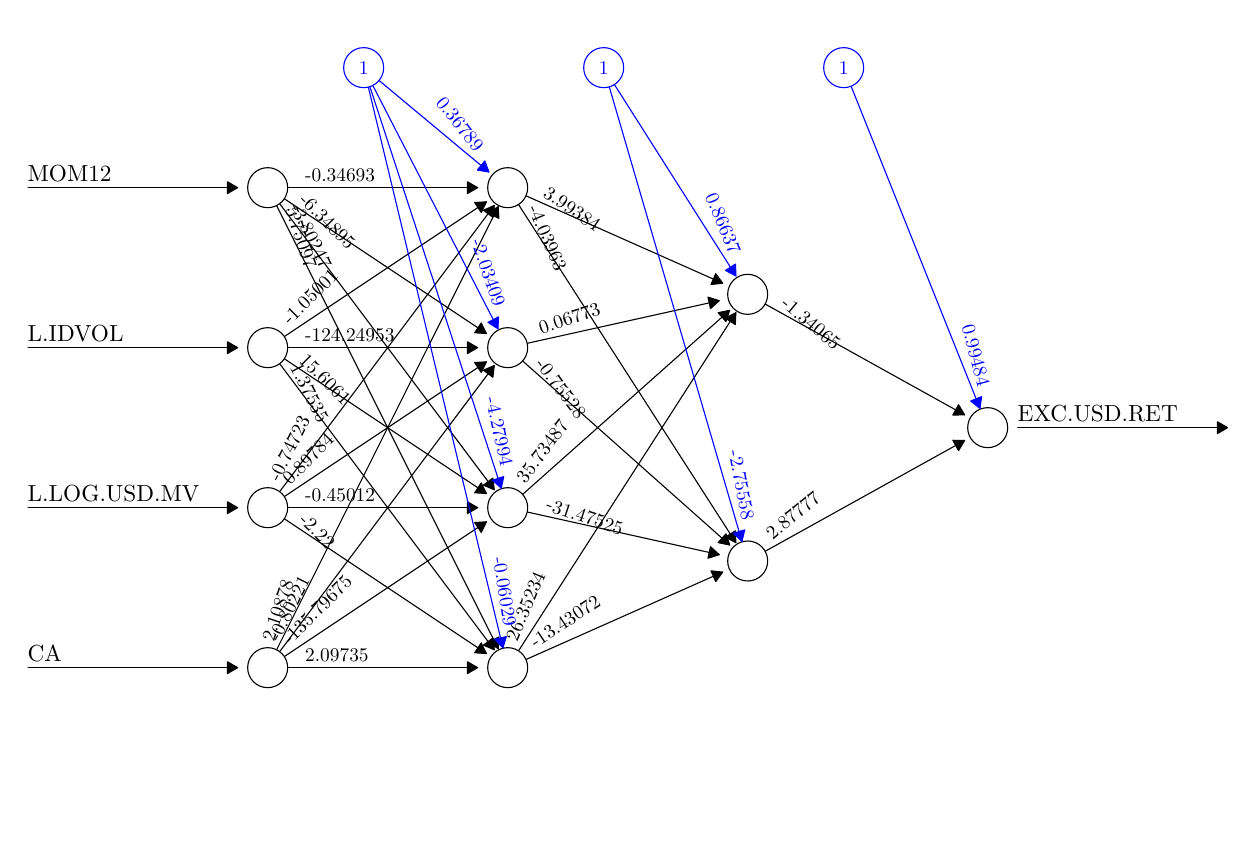
\begin{tikzpicture}[x=1pt,y=1pt]
\definecolor{fillColor}{RGB}{255,255,255}
\path[use as bounding box,fill=fillColor,fill opacity=0.00] (0,0) rectangle (433.62,289.08);
\begin{scope}
\path[clip] (  0.00,  0.00) rectangle (433.62,289.08);
\definecolor{drawColor}{RGB}{0,0,0}

\path[draw=drawColor,line width= 0.4pt,line join=round,line cap=round] ( 86.72, 57.82) --
	(162.61, 57.82);
\definecolor{fillColor}{RGB}{0,0,0}

\path[draw=drawColor,line width= 0.4pt,line join=round,line cap=round,fill=fillColor] (158.91, 55.68) --
	(162.61, 57.82) --
	(158.91, 59.95) --
	cycle;

\node[text=drawColor,anchor=base west,inner sep=0pt, outer sep=0pt, scale=  0.70] at (100.27, 59.95) {2.09735};
\end{scope}
\begin{scope}
\path[clip] (  0.00,  0.00) rectangle (433.62,289.08);
\definecolor{drawColor}{RGB}{0,0,0}

\path[draw=drawColor,line width= 0.4pt,line join=round,line cap=round] ( 86.72, 57.82) --
	(165.78,110.52);
\definecolor{fillColor}{RGB}{0,0,0}

\path[draw=drawColor,line width= 0.4pt,line join=round,line cap=round,fill=fillColor] (163.89,106.70) --
	(165.78,110.52) --
	(161.52,110.25) --
	cycle;

\node[text=drawColor,rotate= 45.00,anchor=base west,inner sep=0pt, outer sep=0pt, scale=  0.70] at ( 94.80, 65.71) {-135.79675};
\end{scope}
\begin{scope}
\path[clip] (  0.00,  0.00) rectangle (433.62,289.08);
\definecolor{drawColor}{RGB}{0,0,0}

\path[draw=drawColor,line width= 0.4pt,line join=round,line cap=round] ( 86.72, 57.82) --
	(168.60,166.98);
\definecolor{fillColor}{RGB}{0,0,0}

\path[draw=drawColor,line width= 0.4pt,line join=round,line cap=round,fill=fillColor] (168.09,162.75) --
	(168.60,166.98) --
	(164.68,165.31) --
	cycle;

\node[text=drawColor,rotate= 63.43,anchor=base west,inner sep=0pt, outer sep=0pt, scale=  0.70] at ( 90.88, 66.85) {-0.80221};
\end{scope}
\begin{scope}
\path[clip] (  0.00,  0.00) rectangle (433.62,289.08);
\definecolor{drawColor}{RGB}{0,0,0}

\path[draw=drawColor,line width= 0.4pt,line join=round,line cap=round] ( 86.72, 57.82) --
	(170.02,224.41);
\definecolor{fillColor}{RGB}{0,0,0}

\path[draw=drawColor,line width= 0.4pt,line join=round,line cap=round,fill=fillColor] (170.28,220.15) --
	(170.02,224.41) --
	(166.46,222.06) --
	cycle;

\node[text=drawColor,rotate= 71.57,anchor=base west,inner sep=0pt, outer sep=0pt, scale=  0.70] at ( 88.98, 67.06) {2.10878};
\end{scope}
\begin{scope}
\path[clip] (  0.00,  0.00) rectangle (433.62,289.08);
\definecolor{drawColor}{RGB}{0,0,0}

\path[draw=drawColor,line width= 0.4pt,line join=round,line cap=round] ( -0.00, 57.82) --
	( 75.88, 57.82);
\definecolor{fillColor}{RGB}{0,0,0}

\path[draw=drawColor,line width= 0.4pt,line join=round,line cap=round,fill=fillColor] ( 72.19, 55.68) --
	( 75.88, 57.82) --
	( 72.19, 59.95) --
	cycle;

\node[text=drawColor,anchor=base west,inner sep=0pt, outer sep=0pt, scale=  0.84] at ( -0.00, 59.95) {CA};
\end{scope}
\begin{scope}
\path[clip] (  0.00,  0.00) rectangle (433.62,289.08);
\definecolor{drawColor}{RGB}{0,0,0}
\definecolor{fillColor}{RGB}{255,255,255}

\path[draw=drawColor,line width= 0.4pt,line join=round,line cap=round,fill=fillColor] ( 86.72, 57.82) circle (  7.23);

\path[draw=drawColor,line width= 0.4pt,line join=round,line cap=round] ( 86.72,115.63) --
	(165.78, 62.93);
\definecolor{fillColor}{RGB}{0,0,0}

\path[draw=drawColor,line width= 0.4pt,line join=round,line cap=round,fill=fillColor] (161.52, 63.20) --
	(165.78, 62.93) --
	(163.89, 66.75) --
	cycle;

\node[text=drawColor,rotate=-45.00,anchor=base west,inner sep=0pt, outer sep=0pt, scale=  0.70] at ( 97.81,110.75) {-2.22};
\end{scope}
\begin{scope}
\path[clip] (  0.00,  0.00) rectangle (433.62,289.08);
\definecolor{drawColor}{RGB}{0,0,0}

\path[draw=drawColor,line width= 0.4pt,line join=round,line cap=round] ( 86.72,115.63) --
	(162.61,115.63);
\definecolor{fillColor}{RGB}{0,0,0}

\path[draw=drawColor,line width= 0.4pt,line join=round,line cap=round,fill=fillColor] (158.91,113.50) --
	(162.61,115.63) --
	(158.91,117.77) --
	cycle;

\node[text=drawColor,anchor=base west,inner sep=0pt, outer sep=0pt, scale=  0.70] at (100.27,117.77) {-0.45012};
\end{scope}
\begin{scope}
\path[clip] (  0.00,  0.00) rectangle (433.62,289.08);
\definecolor{drawColor}{RGB}{0,0,0}

\path[draw=drawColor,line width= 0.4pt,line join=round,line cap=round] ( 86.72,115.63) --
	(165.78,168.34);
\definecolor{fillColor}{RGB}{0,0,0}

\path[draw=drawColor,line width= 0.4pt,line join=round,line cap=round,fill=fillColor] (163.89,164.51) --
	(165.78,168.34) --
	(161.52,168.06) --
	cycle;

\node[text=drawColor,rotate= 45.00,anchor=base west,inner sep=0pt, outer sep=0pt, scale=  0.70] at ( 94.80,123.53) {0.89784};
\end{scope}
\begin{scope}
\path[clip] (  0.00,  0.00) rectangle (433.62,289.08);
\definecolor{drawColor}{RGB}{0,0,0}

\path[draw=drawColor,line width= 0.4pt,line join=round,line cap=round] ( 86.72,115.63) --
	(168.60,224.80);
\definecolor{fillColor}{RGB}{0,0,0}

\path[draw=drawColor,line width= 0.4pt,line join=round,line cap=round,fill=fillColor] (168.09,220.56) --
	(168.60,224.80) --
	(164.68,223.12) --
	cycle;

\node[text=drawColor,rotate= 63.43,anchor=base west,inner sep=0pt, outer sep=0pt, scale=  0.70] at ( 90.88,124.67) {-0.74723};
\end{scope}
\begin{scope}
\path[clip] (  0.00,  0.00) rectangle (433.62,289.08);
\definecolor{drawColor}{RGB}{0,0,0}

\path[draw=drawColor,line width= 0.4pt,line join=round,line cap=round] ( -0.00,115.63) --
	( 75.88,115.63);
\definecolor{fillColor}{RGB}{0,0,0}

\path[draw=drawColor,line width= 0.4pt,line join=round,line cap=round,fill=fillColor] ( 72.19,113.50) --
	( 75.88,115.63) --
	( 72.19,117.77) --
	cycle;

\node[text=drawColor,anchor=base west,inner sep=0pt, outer sep=0pt, scale=  0.84] at ( -0.00,117.77) {L.LOG.USD.MV};
\end{scope}
\begin{scope}
\path[clip] (  0.00,  0.00) rectangle (433.62,289.08);
\definecolor{drawColor}{RGB}{0,0,0}
\definecolor{fillColor}{RGB}{255,255,255}

\path[draw=drawColor,line width= 0.4pt,line join=round,line cap=round,fill=fillColor] ( 86.72,115.63) circle (  7.23);

\path[draw=drawColor,line width= 0.4pt,line join=round,line cap=round] ( 86.72,173.45) --
	(168.60, 64.28);
\definecolor{fillColor}{RGB}{0,0,0}

\path[draw=drawColor,line width= 0.4pt,line join=round,line cap=round,fill=fillColor] (164.68, 65.96) --
	(168.60, 64.28) --
	(168.09, 68.52) --
	cycle;

\node[text=drawColor,rotate=-63.43,anchor=base west,inner sep=0pt, outer sep=0pt, scale=  0.70] at ( 94.69,166.32) {1.37535};
\end{scope}
\begin{scope}
\path[clip] (  0.00,  0.00) rectangle (433.62,289.08);
\definecolor{drawColor}{RGB}{0,0,0}

\path[draw=drawColor,line width= 0.4pt,line join=round,line cap=round] ( 86.72,173.45) --
	(165.78,120.74);
\definecolor{fillColor}{RGB}{0,0,0}

\path[draw=drawColor,line width= 0.4pt,line join=round,line cap=round,fill=fillColor] (161.52,121.02) --
	(165.78,120.74) --
	(163.89,124.57) --
	cycle;

\node[text=drawColor,rotate=-45.00,anchor=base west,inner sep=0pt, outer sep=0pt, scale=  0.70] at ( 97.81,168.57) {15.6061};
\end{scope}
\begin{scope}
\path[clip] (  0.00,  0.00) rectangle (433.62,289.08);
\definecolor{drawColor}{RGB}{0,0,0}

\path[draw=drawColor,line width= 0.4pt,line join=round,line cap=round] ( 86.72,173.45) --
	(162.61,173.45);
\definecolor{fillColor}{RGB}{0,0,0}

\path[draw=drawColor,line width= 0.4pt,line join=round,line cap=round,fill=fillColor] (158.91,171.31) --
	(162.61,173.45) --
	(158.91,175.58) --
	cycle;

\node[text=drawColor,anchor=base west,inner sep=0pt, outer sep=0pt, scale=  0.70] at (100.27,175.58) {-124.24953};
\end{scope}
\begin{scope}
\path[clip] (  0.00,  0.00) rectangle (433.62,289.08);
\definecolor{drawColor}{RGB}{0,0,0}

\path[draw=drawColor,line width= 0.4pt,line join=round,line cap=round] ( 86.72,173.45) --
	(165.78,226.15);
\definecolor{fillColor}{RGB}{0,0,0}

\path[draw=drawColor,line width= 0.4pt,line join=round,line cap=round,fill=fillColor] (163.89,222.33) --
	(165.78,226.15) --
	(161.52,225.88) --
	cycle;

\node[text=drawColor,rotate= 45.00,anchor=base west,inner sep=0pt, outer sep=0pt, scale=  0.70] at ( 94.80,181.34) {-1.05001};
\end{scope}
\begin{scope}
\path[clip] (  0.00,  0.00) rectangle (433.62,289.08);
\definecolor{drawColor}{RGB}{0,0,0}

\path[draw=drawColor,line width= 0.4pt,line join=round,line cap=round] ( -0.00,173.45) --
	( 75.88,173.45);
\definecolor{fillColor}{RGB}{0,0,0}

\path[draw=drawColor,line width= 0.4pt,line join=round,line cap=round,fill=fillColor] ( 72.19,171.31) --
	( 75.88,173.45) --
	( 72.19,175.58) --
	cycle;

\node[text=drawColor,anchor=base west,inner sep=0pt, outer sep=0pt, scale=  0.84] at ( -0.00,175.58) {L.IDVOL};
\end{scope}
\begin{scope}
\path[clip] (  0.00,  0.00) rectangle (433.62,289.08);
\definecolor{drawColor}{RGB}{0,0,0}
\definecolor{fillColor}{RGB}{255,255,255}

\path[draw=drawColor,line width= 0.4pt,line join=round,line cap=round,fill=fillColor] ( 86.72,173.45) circle (  7.23);

\path[draw=drawColor,line width= 0.4pt,line join=round,line cap=round] ( 86.72,231.26) --
	(170.02, 64.67);
\definecolor{fillColor}{RGB}{0,0,0}

\path[draw=drawColor,line width= 0.4pt,line join=round,line cap=round,fill=fillColor] (166.46, 67.02) --
	(170.02, 64.67) --
	(170.28, 68.93) --
	cycle;

\node[text=drawColor,rotate=-71.57,anchor=base west,inner sep=0pt, outer sep=0pt, scale=  0.70] at ( 93.03,223.37) {5.75097};
\end{scope}
\begin{scope}
\path[clip] (  0.00,  0.00) rectangle (433.62,289.08);
\definecolor{drawColor}{RGB}{0,0,0}

\path[draw=drawColor,line width= 0.4pt,line join=round,line cap=round] ( 86.72,231.26) --
	(168.60,122.10);
\definecolor{fillColor}{RGB}{0,0,0}

\path[draw=drawColor,line width= 0.4pt,line join=round,line cap=round,fill=fillColor] (164.68,123.77) --
	(168.60,122.10) --
	(168.09,126.33) --
	cycle;

\node[text=drawColor,rotate=-63.43,anchor=base west,inner sep=0pt, outer sep=0pt, scale=  0.70] at ( 94.69,224.14) {-3.80247};
\end{scope}
\begin{scope}
\path[clip] (  0.00,  0.00) rectangle (433.62,289.08);
\definecolor{drawColor}{RGB}{0,0,0}

\path[draw=drawColor,line width= 0.4pt,line join=round,line cap=round] ( 86.72,231.26) --
	(165.78,178.56);
\definecolor{fillColor}{RGB}{0,0,0}

\path[draw=drawColor,line width= 0.4pt,line join=round,line cap=round,fill=fillColor] (161.52,178.83) --
	(165.78,178.56) --
	(163.89,182.38) --
	cycle;

\node[text=drawColor,rotate=-45.00,anchor=base west,inner sep=0pt, outer sep=0pt, scale=  0.70] at ( 97.81,226.39) {-6.34895};
\end{scope}
\begin{scope}
\path[clip] (  0.00,  0.00) rectangle (433.62,289.08);
\definecolor{drawColor}{RGB}{0,0,0}

\path[draw=drawColor,line width= 0.4pt,line join=round,line cap=round] ( 86.72,231.26) --
	(162.61,231.26);
\definecolor{fillColor}{RGB}{0,0,0}

\path[draw=drawColor,line width= 0.4pt,line join=round,line cap=round,fill=fillColor] (158.91,229.13) --
	(162.61,231.26) --
	(158.91,233.40) --
	cycle;

\node[text=drawColor,anchor=base west,inner sep=0pt, outer sep=0pt, scale=  0.70] at (100.27,233.40) {-0.34693};
\end{scope}
\begin{scope}
\path[clip] (  0.00,  0.00) rectangle (433.62,289.08);
\definecolor{drawColor}{RGB}{0,0,0}

\path[draw=drawColor,line width= 0.4pt,line join=round,line cap=round] ( -0.00,231.26) --
	( 75.88,231.26);
\definecolor{fillColor}{RGB}{0,0,0}

\path[draw=drawColor,line width= 0.4pt,line join=round,line cap=round,fill=fillColor] ( 72.19,229.13) --
	( 75.88,231.26) --
	( 72.19,233.40) --
	cycle;

\node[text=drawColor,anchor=base west,inner sep=0pt, outer sep=0pt, scale=  0.84] at ( -0.00,233.40) {MOM12};
\end{scope}
\begin{scope}
\path[clip] (  0.00,  0.00) rectangle (433.62,289.08);
\definecolor{drawColor}{RGB}{0,0,0}
\definecolor{fillColor}{RGB}{255,255,255}

\path[draw=drawColor,line width= 0.4pt,line join=round,line cap=round,fill=fillColor] ( 86.72,231.26) circle (  7.23);

\path[draw=drawColor,line width= 0.4pt,line join=round,line cap=round] (173.45, 57.82) --
	(251.15, 92.35);
\definecolor{fillColor}{RGB}{0,0,0}

\path[draw=drawColor,line width= 0.4pt,line join=round,line cap=round,fill=fillColor] (248.64, 88.90) --
	(251.15, 92.35) --
	(246.91, 92.80) --
	cycle;

\node[text=drawColor,rotate= 33.69,anchor=base west,inner sep=0pt, outer sep=0pt, scale=  0.70] at (183.54, 64.60) {-13.43072};
\end{scope}
\begin{scope}
\path[clip] (  0.00,  0.00) rectangle (433.62,289.08);
\definecolor{drawColor}{RGB}{0,0,0}

\path[draw=drawColor,line width= 0.4pt,line join=round,line cap=round] (173.45, 57.82) --
	(255.90,186.08);
\definecolor{fillColor}{RGB}{0,0,0}

\path[draw=drawColor,line width= 0.4pt,line join=round,line cap=round,fill=fillColor] (255.70,181.81) --
	(255.90,186.08) --
	(252.11,184.12) --
	cycle;

\node[text=drawColor,rotate= 66.80,anchor=base west,inner sep=0pt, outer sep=0pt, scale=  0.70] at (176.82, 66.96) {26.35234};
\end{scope}
\begin{scope}
\path[clip] (  0.00,  0.00) rectangle (433.62,289.08);
\definecolor{drawColor}{RGB}{0,0,0}
\definecolor{fillColor}{RGB}{255,255,255}

\path[draw=drawColor,line width= 0.4pt,line join=round,line cap=round,fill=fillColor] (173.45, 57.82) circle (  7.23);

\path[draw=drawColor,line width= 0.4pt,line join=round,line cap=round] (173.45,115.63) --
	(249.89, 98.65);
\definecolor{fillColor}{RGB}{0,0,0}

\path[draw=drawColor,line width= 0.4pt,line join=round,line cap=round,fill=fillColor] (245.82, 97.36) --
	(249.89, 98.65) --
	(246.74,101.53) --
	cycle;

\node[text=drawColor,rotate=-18.43,anchor=base west,inner sep=0pt, outer sep=0pt, scale=  0.70] at (186.98,114.80) {-31.47525};
\end{scope}
\begin{scope}
\path[clip] (  0.00,  0.00) rectangle (433.62,289.08);
\definecolor{drawColor}{RGB}{0,0,0}

\path[draw=drawColor,line width= 0.4pt,line join=round,line cap=round] (173.45,115.63) --
	(253.67,186.94);
\definecolor{fillColor}{RGB}{0,0,0}

\path[draw=drawColor,line width= 0.4pt,line join=round,line cap=round,fill=fillColor] (252.32,182.89) --
	(253.67,186.94) --
	(249.49,186.08) --
	cycle;

\node[text=drawColor,rotate= 53.13,anchor=base west,inner sep=0pt, outer sep=0pt, scale=  0.70] at (179.87,124.14) {35.73487};
\end{scope}
\begin{scope}
\path[clip] (  0.00,  0.00) rectangle (433.62,289.08);
\definecolor{drawColor}{RGB}{0,0,0}
\definecolor{fillColor}{RGB}{255,255,255}

\path[draw=drawColor,line width= 0.4pt,line join=round,line cap=round,fill=fillColor] (173.45,115.63) circle (  7.23);

\path[draw=drawColor,line width= 0.4pt,line join=round,line cap=round] (173.45,173.45) --
	(253.67,102.14);
\definecolor{fillColor}{RGB}{0,0,0}

\path[draw=drawColor,line width= 0.4pt,line join=round,line cap=round,fill=fillColor] (249.49,103.00) --
	(253.67,102.14) --
	(252.32,106.19) --
	cycle;

\node[text=drawColor,rotate=-53.13,anchor=base west,inner sep=0pt, outer sep=0pt, scale=  0.70] at (183.29,167.50) {-0.75528};
\end{scope}
\begin{scope}
\path[clip] (  0.00,  0.00) rectangle (433.62,289.08);
\definecolor{drawColor}{RGB}{0,0,0}

\path[draw=drawColor,line width= 0.4pt,line join=round,line cap=round] (173.45,173.45) --
	(249.89,190.43);
\definecolor{fillColor}{RGB}{0,0,0}

\path[draw=drawColor,line width= 0.4pt,line join=round,line cap=round,fill=fillColor] (246.74,187.55) --
	(249.89,190.43) --
	(245.82,191.72) --
	cycle;

\node[text=drawColor,rotate= 18.43,anchor=base west,inner sep=0pt, outer sep=0pt, scale=  0.70] at (185.63,178.33) {0.06773};
\end{scope}
\begin{scope}
\path[clip] (  0.00,  0.00) rectangle (433.62,289.08);
\definecolor{drawColor}{RGB}{0,0,0}
\definecolor{fillColor}{RGB}{255,255,255}

\path[draw=drawColor,line width= 0.4pt,line join=round,line cap=round,fill=fillColor] (173.45,173.45) circle (  7.23);

\path[draw=drawColor,line width= 0.4pt,line join=round,line cap=round] (173.45,231.26) --
	(255.90,103.00);
\definecolor{fillColor}{RGB}{0,0,0}

\path[draw=drawColor,line width= 0.4pt,line join=round,line cap=round,fill=fillColor] (252.11,104.96) --
	(255.90,103.00) --
	(255.70,107.27) --
	cycle;

\node[text=drawColor,rotate=-66.80,anchor=base west,inner sep=0pt, outer sep=0pt, scale=  0.70] at (180.75,223.80) {-4.03963};
\end{scope}
\begin{scope}
\path[clip] (  0.00,  0.00) rectangle (433.62,289.08);
\definecolor{drawColor}{RGB}{0,0,0}

\path[draw=drawColor,line width= 0.4pt,line join=round,line cap=round] (173.45,231.26) --
	(251.15,196.73);
\definecolor{fillColor}{RGB}{0,0,0}

\path[draw=drawColor,line width= 0.4pt,line join=round,line cap=round,fill=fillColor] (246.91,196.28) --
	(251.15,196.73) --
	(248.64,200.18) --
	cycle;

\node[text=drawColor,rotate=-33.69,anchor=base west,inner sep=0pt, outer sep=0pt, scale=  0.70] at (185.91,228.03) {3.99384};
\end{scope}
\begin{scope}
\path[clip] (  0.00,  0.00) rectangle (433.62,289.08);
\definecolor{drawColor}{RGB}{0,0,0}
\definecolor{fillColor}{RGB}{255,255,255}

\path[draw=drawColor,line width= 0.4pt,line join=round,line cap=round,fill=fillColor] (173.45,231.26) circle (  7.23);

\path[draw=drawColor,line width= 0.4pt,line join=round,line cap=round] (260.17, 96.36) --
	(338.57,139.91);
\definecolor{fillColor}{RGB}{0,0,0}

\path[draw=drawColor,line width= 0.4pt,line join=round,line cap=round,fill=fillColor] (336.37,136.25) --
	(338.57,139.91) --
	(334.30,139.98) --
	cycle;

\node[text=drawColor,rotate= 39.81,anchor=base west,inner sep=0pt, outer sep=0pt, scale=  0.70] at (269.22,103.78) {2.87777};
\end{scope}
\begin{scope}
\path[clip] (  0.00,  0.00) rectangle (433.62,289.08);
\definecolor{drawColor}{RGB}{0,0,0}
\definecolor{fillColor}{RGB}{255,255,255}

\path[draw=drawColor,line width= 0.4pt,line join=round,line cap=round,fill=fillColor] (260.17, 96.36) circle (  7.23);

\path[draw=drawColor,line width= 0.4pt,line join=round,line cap=round] (260.17,192.72) --
	(338.57,149.17);
\definecolor{fillColor}{RGB}{0,0,0}

\path[draw=drawColor,line width= 0.4pt,line join=round,line cap=round,fill=fillColor] (334.30,149.10) --
	(338.57,149.17) --
	(336.37,152.83) --
	cycle;

\node[text=drawColor,rotate=-39.81,anchor=base west,inner sep=0pt, outer sep=0pt, scale=  0.70] at (271.95,188.58) {-1.34065};
\end{scope}
\begin{scope}
\path[clip] (  0.00,  0.00) rectangle (433.62,289.08);
\definecolor{drawColor}{RGB}{0,0,0}
\definecolor{fillColor}{RGB}{255,255,255}

\path[draw=drawColor,line width= 0.4pt,line join=round,line cap=round,fill=fillColor] (260.17,192.72) circle (  7.23);

\path[draw=drawColor,line width= 0.4pt,line join=round,line cap=round] (357.74,144.54) --
	(433.62,144.54);
\definecolor{fillColor}{RGB}{0,0,0}

\path[draw=drawColor,line width= 0.4pt,line join=round,line cap=round,fill=fillColor] (429.92,142.41) --
	(433.62,144.54) --
	(429.92,146.67) --
	cycle;

\node[text=drawColor,anchor=base west,inner sep=0pt, outer sep=0pt, scale=  0.84] at (357.74,146.67) {EXC.USD.RET};
\end{scope}
\begin{scope}
\path[clip] (  0.00,  0.00) rectangle (433.62,289.08);
\definecolor{drawColor}{RGB}{0,0,0}
\definecolor{fillColor}{RGB}{255,255,255}

\path[draw=drawColor,line width= 0.4pt,line join=round,line cap=round,fill=fillColor] (346.90,144.54) circle (  7.23);
\definecolor{drawColor}{RGB}{0,0,255}

\path[draw=drawColor,line width= 0.4pt,line join=round,line cap=round] (121.41,274.63) --
	(171.74, 64.95);
\definecolor{fillColor}{RGB}{0,0,255}

\path[draw=drawColor,line width= 0.4pt,line join=round,line cap=round,fill=fillColor] (168.80, 68.05) --
	(171.74, 64.95) --
	(172.95, 69.04) --
	cycle;

\node[text=drawColor,rotate=-80.91,anchor=base east,inner sep=0pt, outer sep=0pt, scale=  0.70] at (172.13, 72.43) {-0.06029};
\end{scope}
\begin{scope}
\path[clip] (  0.00,  0.00) rectangle (433.62,289.08);
\definecolor{drawColor}{RGB}{0,0,255}

\path[draw=drawColor,line width= 0.4pt,line join=round,line cap=round] (121.41,274.63) --
	(171.14,122.69);
\definecolor{fillColor}{RGB}{0,0,255}

\path[draw=drawColor,line width= 0.4pt,line join=round,line cap=round,fill=fillColor] (167.96,125.54) --
	(171.14,122.69) --
	(172.02,126.87) --
	cycle;

\node[text=drawColor,rotate=-77.69,anchor=base east,inner sep=0pt, outer sep=0pt, scale=  0.70] at (170.91,130.21) {-4.27994};
\end{scope}
\begin{scope}
\path[clip] (  0.00,  0.00) rectangle (433.62,289.08);
\definecolor{drawColor}{RGB}{0,0,255}

\path[draw=drawColor,line width= 0.4pt,line join=round,line cap=round] (121.41,274.63) --
	(169.93,180.28);
\definecolor{fillColor}{RGB}{0,0,255}

\path[draw=drawColor,line width= 0.4pt,line join=round,line cap=round,fill=fillColor] (166.34,182.60) --
	(169.93,180.28) --
	(170.14,184.55) --
	cycle;

\node[text=drawColor,rotate=-71.08,anchor=base east,inner sep=0pt, outer sep=0pt, scale=  0.70] at (168.43,187.81) {-2.03409};
\end{scope}
\begin{scope}
\path[clip] (  0.00,  0.00) rectangle (433.62,289.08);
\definecolor{drawColor}{RGB}{0,0,255}

\path[draw=drawColor,line width= 0.4pt,line join=round,line cap=round] (121.41,274.63) --
	(166.68,236.91);
\definecolor{fillColor}{RGB}{0,0,255}

\path[draw=drawColor,line width= 0.4pt,line join=round,line cap=round,fill=fillColor] (162.47,237.63) --
	(166.68,236.91) --
	(165.20,240.91) --
	cycle;

\node[text=drawColor,rotate=-51.34,anchor=base east,inner sep=0pt, outer sep=0pt, scale=  0.70] at (161.57,243.88) {0.36789};
\end{scope}
\begin{scope}
\path[clip] (  0.00,  0.00) rectangle (433.62,289.08);
\definecolor{drawColor}{RGB}{0,0,255}
\definecolor{fillColor}{RGB}{255,255,255}

\path[draw=drawColor,line width= 0.4pt,line join=round,line cap=round,fill=fillColor] (121.41,274.63) circle (  7.23);

\node[text=drawColor,anchor=base,inner sep=0pt, outer sep=0pt, scale=  0.70] at (121.41,272.22) {1};

\path[draw=drawColor,line width= 0.4pt,line join=round,line cap=round] (208.14,274.63) --
	(258.10,103.45);
\definecolor{fillColor}{RGB}{0,0,255}

\path[draw=drawColor,line width= 0.4pt,line join=round,line cap=round,fill=fillColor] (255.02,106.40) --
	(258.10,103.45) --
	(259.11,107.60) --
	cycle;

\node[text=drawColor,rotate=-78.99,anchor=base east,inner sep=0pt, outer sep=0pt, scale=  0.70] at (258.13,110.96) {-2.75558};
\end{scope}
\begin{scope}
\path[clip] (  0.00,  0.00) rectangle (433.62,289.08);
\definecolor{drawColor}{RGB}{0,0,255}

\path[draw=drawColor,line width= 0.4pt,line join=round,line cap=round] (208.14,274.63) --
	(255.94,199.37);
\definecolor{fillColor}{RGB}{0,0,255}

\path[draw=drawColor,line width= 0.4pt,line join=round,line cap=round,fill=fillColor] (252.16,201.35) --
	(255.94,199.37) --
	(255.76,203.64) --
	cycle;

\node[text=drawColor,rotate=-67.05,anchor=base east,inner sep=0pt, outer sep=0pt, scale=  0.70] at (253.68,206.86) {0.86637};
\end{scope}
\begin{scope}
\path[clip] (  0.00,  0.00) rectangle (433.62,289.08);
\definecolor{drawColor}{RGB}{0,0,255}
\definecolor{fillColor}{RGB}{255,255,255}

\path[draw=drawColor,line width= 0.4pt,line join=round,line cap=round,fill=fillColor] (208.14,274.63) circle (  7.23);

\node[text=drawColor,anchor=base,inner sep=0pt, outer sep=0pt, scale=  0.70] at (208.14,272.22) {1};

\path[draw=drawColor,line width= 0.4pt,line join=round,line cap=round] (294.86,274.63) --
	(344.10,151.52);
\definecolor{fillColor}{RGB}{0,0,255}

\path[draw=drawColor,line width= 0.4pt,line join=round,line cap=round,fill=fillColor] (340.75,154.16) --
	(344.10,151.52) --
	(344.71,155.75) --
	cycle;

\node[text=drawColor,rotate=-75.07,anchor=base east,inner sep=0pt, outer sep=0pt, scale=  0.70] at (343.37,159.06) {0.99484};
\end{scope}
\begin{scope}
\path[clip] (  0.00,  0.00) rectangle (433.62,289.08);
\definecolor{drawColor}{RGB}{0,0,255}
\definecolor{fillColor}{RGB}{255,255,255}

\path[draw=drawColor,line width= 0.4pt,line join=round,line cap=round,fill=fillColor] (294.86,274.63) circle (  7.23);

\node[text=drawColor,anchor=base,inner sep=0pt, outer sep=0pt, scale=  0.70] at (294.86,272.22) {1};
\end{scope}
\end{tikzpicture}
